\section{Álgebra y Funciones}
\def\svgwidth{\columnwidth}

\subsection{Factorización}
$ (a \pm b \pm c)^2 = a^2 + b^2 + c^2 \pm 2ab \pm 2ac \pm 2bc $\\
$(a \pm b)^3 = a^3 \pm 3a^2b + 3ab^2 \pm b^3$\\
$ a^3 \pm b^3 = (a \pm b)(a^2 \mp ab + b^2)$\\
$ (x + p)(x + q) = x^2 + x(p + q) + pq $\\
$ a (a + b + 1) = a^2 + ab + a $\\

\subsection{Dominio y Recorrido}
El \textit{dominio} de definición de una función es el conjunto de valores de entrada, o argumentos, para la cual una cierta función está definida. Análogamente, el conjunto de valores de salida, es denominado \textit{rango o imagen}, que es un subconjunto del codominio de la función. Gráficamente, el dominio está representado por el eje x de un plano cartesiano, y el rango por el eje y.\\

Para una función $f: X \rightarrow Y$, donde el conjunto $X$ es el dominio, e $Y$ el codominio, el rango está definido por $\left\{ f(x) | x \in X \right\}$, y siempre es un subconjunto de $Y$. Cuando el rango es todo el conjunto del codominio, la función es sobreyectiva.\\

El rango también se puede encontrar en el dominio de la función inversa, es decir, invirtiendo la variable independiente con la dependiente, y resolviendo el dominio.\\

\subsection{Inyectividad y Epiyectividad}
Una función $f(x)$ es \textit{inyectiva} cuando,
$\forall a,b \in X, \;\; f(a)=f(b) \Rightarrow a=b$
, es decir cuando nunca mapea elementos distintos de su \textit{Dominio} a un mismo elemento del \textit{Codominio}.

Análogamente, se dice que una función f(x) es \textit{sobreyectiva}, o epiyectiva cuando, $\forall y \in Y, \, \exists x \in X, \;\; f(x)=y$, es decir, que para cada elemento $y$ en el codominio $Y$, hay al menos un elemento $x$ en el dominio $X$ de forma que $f(x) = y$.\\
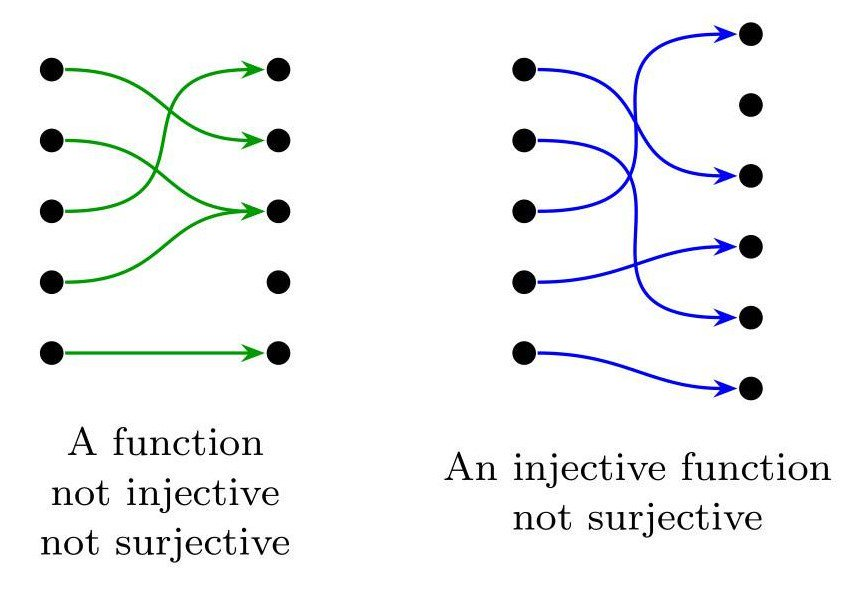
\includegraphics[width=\columnwidth]{inyectividad}\\
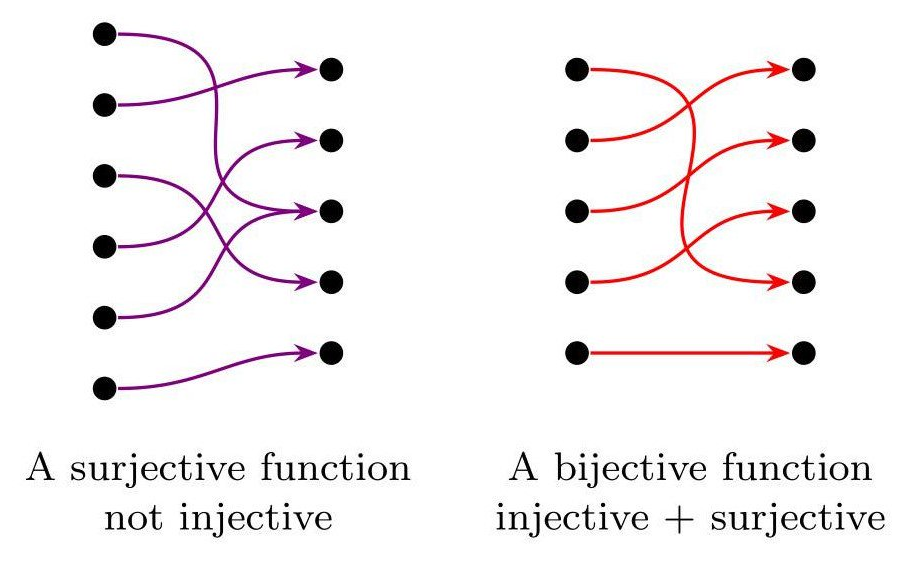
\includegraphics[width=\columnwidth]{sobreyectividad}
\subsection{Función Afín}
Una función afin tiene una \textbf{forma principal} de $y = mx + n$, donde se denomina lineal si $n=0$, y una \textbf{forma general} de $ax + by = 0$.\\
Para la forma general, $m = -\frac{a}{b}$ y $n = -\frac{c}{b}.$\\
Punto pendiente: $y - y_1 = m(x - x_1)$\\
Dos Puntos: $\frac{y-y_1}{x-x_1} = \frac{y_2-y_1}{x_2-x_1}$\\
Distancia punto-recta: $\frac{|ax_0+by_0+c|}{\sqrt{a^2+b^2}}.$\\
\textit{Nota:} $m = \tan \alpha$

\subsection{Función Cuadrática}
Formatos:\\
$f(x) = a x^2 + b x + c \,\!$ llamada \textbf{forma estándar}\\
$f(x) = a(x - r_1)(x - r_2)\,\!$, llamada \textbf{forma factorizada}, con $r_1$ y $r_2$ raíces.\\
$f(x) = a(x - h)^2 + k \,\!$, llamada \textbf{forma de vértice}, con un vértice $(h, k)$.\\

Vértice: $(\frac{-b}{2a}),-\frac{b^2-4ac}{4a})$\\
$x_1 + x_2 = \frac{-b}{a}$\\
$x_1 \cdot x_2 = \frac{c}{a}$\\

\subsection{Función Exponencial}
Una función exponencial usualmente está descrita en la forma $(x) = ab^x$ con b un número real positivo y $x$ exponente. De forma simplificada $f(x) = b^x$, donde si $b > 1$ la función es creciente (hacia la derecha) y cuando $0 < b < 1$ la función es decreciente.\\

\subsection{Función Potencia}
Clase de la que pertenece la función cuadrática, está definida en forma general por $f(x) = ax^n$ con $n \in \mathbb{N} - \{1\}$ y $a \in \mathbb{R}$.

Cuando $n$ es \textbf{par}, entonces la función toma la forma de una parábola, y cuando es \textbf{impar}, toma una forma similar a la cúbica.

\subsection{Función Logarítmica}
Siguen la forma general $f(x) = log_b{x}$, y son inversas de las funciones exponenciales, siendo simétricas con respecto a $y = x$.\\
\begin{minipage}[c]{\columnwidth}
    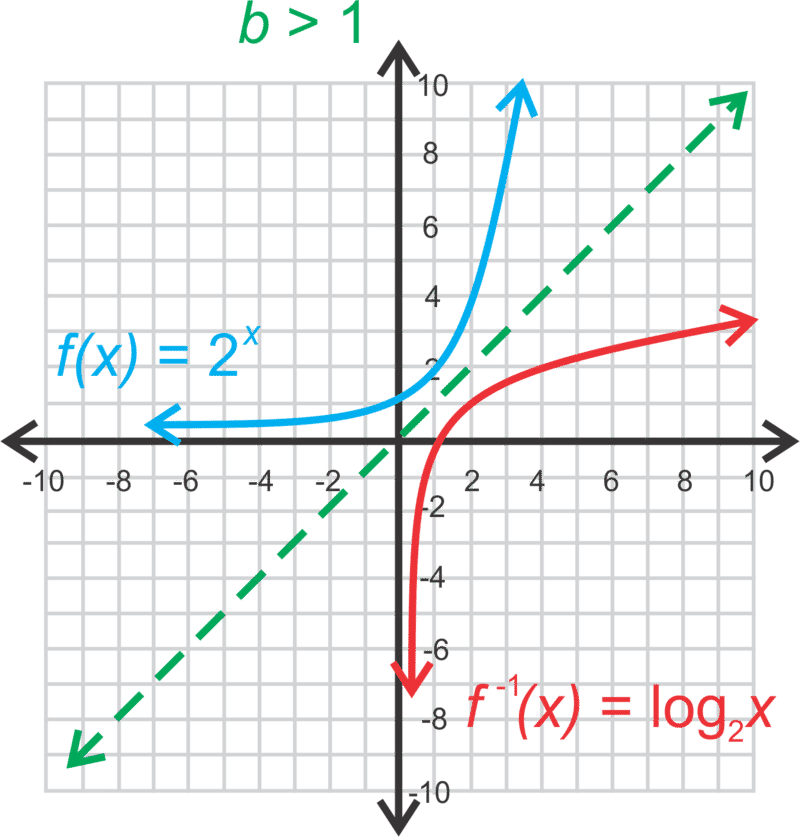
\includegraphics[width=0.49\columnwidth]{funcionlogaritmica1}
    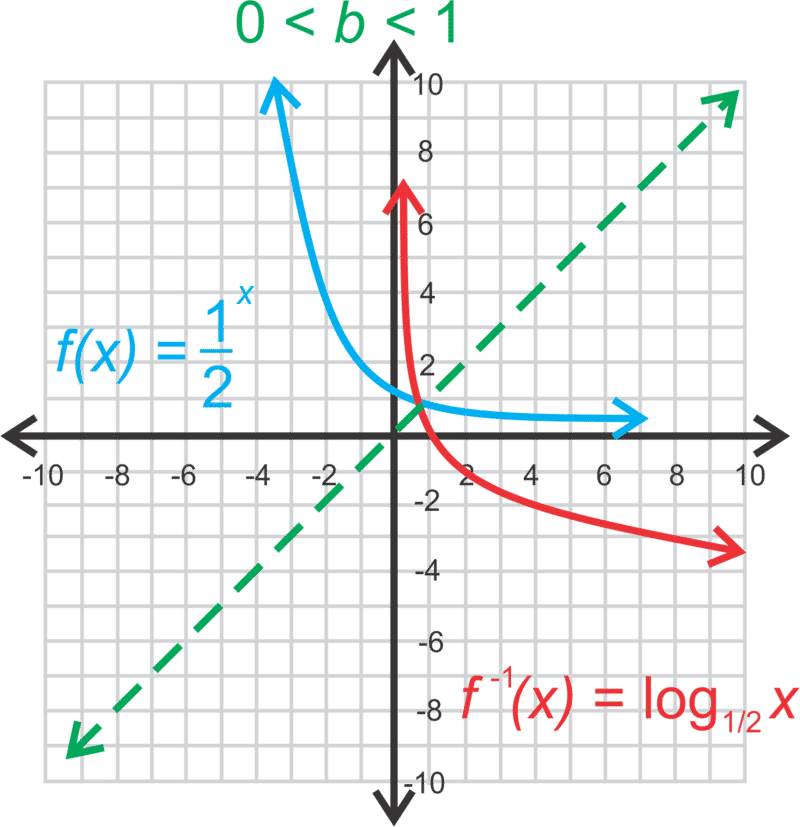
\includegraphics[width=0.49\columnwidth]{funcionlogaritmica2}
\end{minipage}

\subsection{Sistemas de Ecuaciones Lineales}
Un \textbf{sistema de ecuaciones lineales} o sistema lineal es una colección de dos o mas ecuaciones lineales (nótese, uso no análogo a afín/lineal) que involucra el mismo conjunto de variables. Una \textbf{solución} a tal sistema es una asignación de valores a las variables de forma de que todas se encuentren satisfechas.\\

\textit{Nota:} Formalmente, se define como forma general:\\
$a_{11} x_1 + a_{12} x_2  + \cdots + a_{1n} x_n  = b_1 \\
    a_{21} x_1 + a_{22} x_2  + \cdots + a_{2n} x_n  = b_2 \\
    \ \ \vdots\\
    a_{m1} x_1 + a_{m2} x_2  + \cdots + a_{mn} x_n  = b_ m$\\
    Donde $x_1, x_2,\ldots,x_n$ son las incógnitas, $a_{11},a_{12},\ldots,a_{mn}$ los coeficientes, y $b_1,b_2,\ldots,b_m$ términos constantes.\\

    Aparte de esta forma, un sistema lineal puede ser representado como una combinación lineal de una ecuación vectorial, una ecuación de matrices (por equivalencia) y una representación geométrica de \textit{n-}planos.
\subsubsection{Interpretación Geométrica}
Un sistema de ecuaciones lineales con dos incógnitas y dos ecuaciones pueden representarse como \textbf{dos rectas en el plano}, con sus respectivas intersecciones correspondiendo a las soluciones al sistema.
\textit{Nota:} Para tres variables, cada ecuación linear determina un plano en espacio tridimensional, y para \textit{n} variables, cada ecuación lineal determina un hiperplano (un subespacio con una dimensión una menor que la de su espacio) en un espacio \textit{n-}dimensional.
\subsubsection{Soluciones}
Según la cantidad de soluciones, un sistema de ecuaciones lineales (en este caso. $2\times2$) puede ser clasificado en:\\

\textit{Compatible determinado:} Una solución, es decir, las rectas son secantes entre ellas (un punto de intersección).\\
\textit{Compatible indeterminado:} Infinitas soluciones, es decir, las rectas son coincidentes.\\
\textit{Incompatible:} Ninguna solución, ocurre cuando las rectas son paralelas (igual pendiente).\\